\section{The Workflow}
\label{sec.framework}

The proposed workflow uses RNA-seq read counts, representing gene
expression levels, as input data. More precisely, it uses $n_0$ gene
expression profiles of an organism, measured for $m$ different
genotypes under control and treatment conditions, and $r$ biological
replicates. This raw data is represented as a matrix $D_0 \in
{\mathbb{N}_0}^{n_0 \times 2mr}$. In order to discover key genes and
their interaction with phenotypes related to treatment tolerance, the
approach also requires a set of $p$ phenotypic traits, measured for
the $m$ genotypes. The phenotypic data is seen as a matrix $P \in
\mathbb{R}^{2m \times p}$ containing two phenotypic values per
genotype, one under control condition and a second one under treatment
condition. The proposed workflow is depicted in
Figure~\ref{fig:flow_chart}. This section explains the five
macro-processes (A)-(E) of the proposed workflow. In comparison with
WGCNA, it adds the macro-step (D) and generalizes macro-steps (A)-(C).

% flow chart
\begin{figure}[htpb]
  \centering
    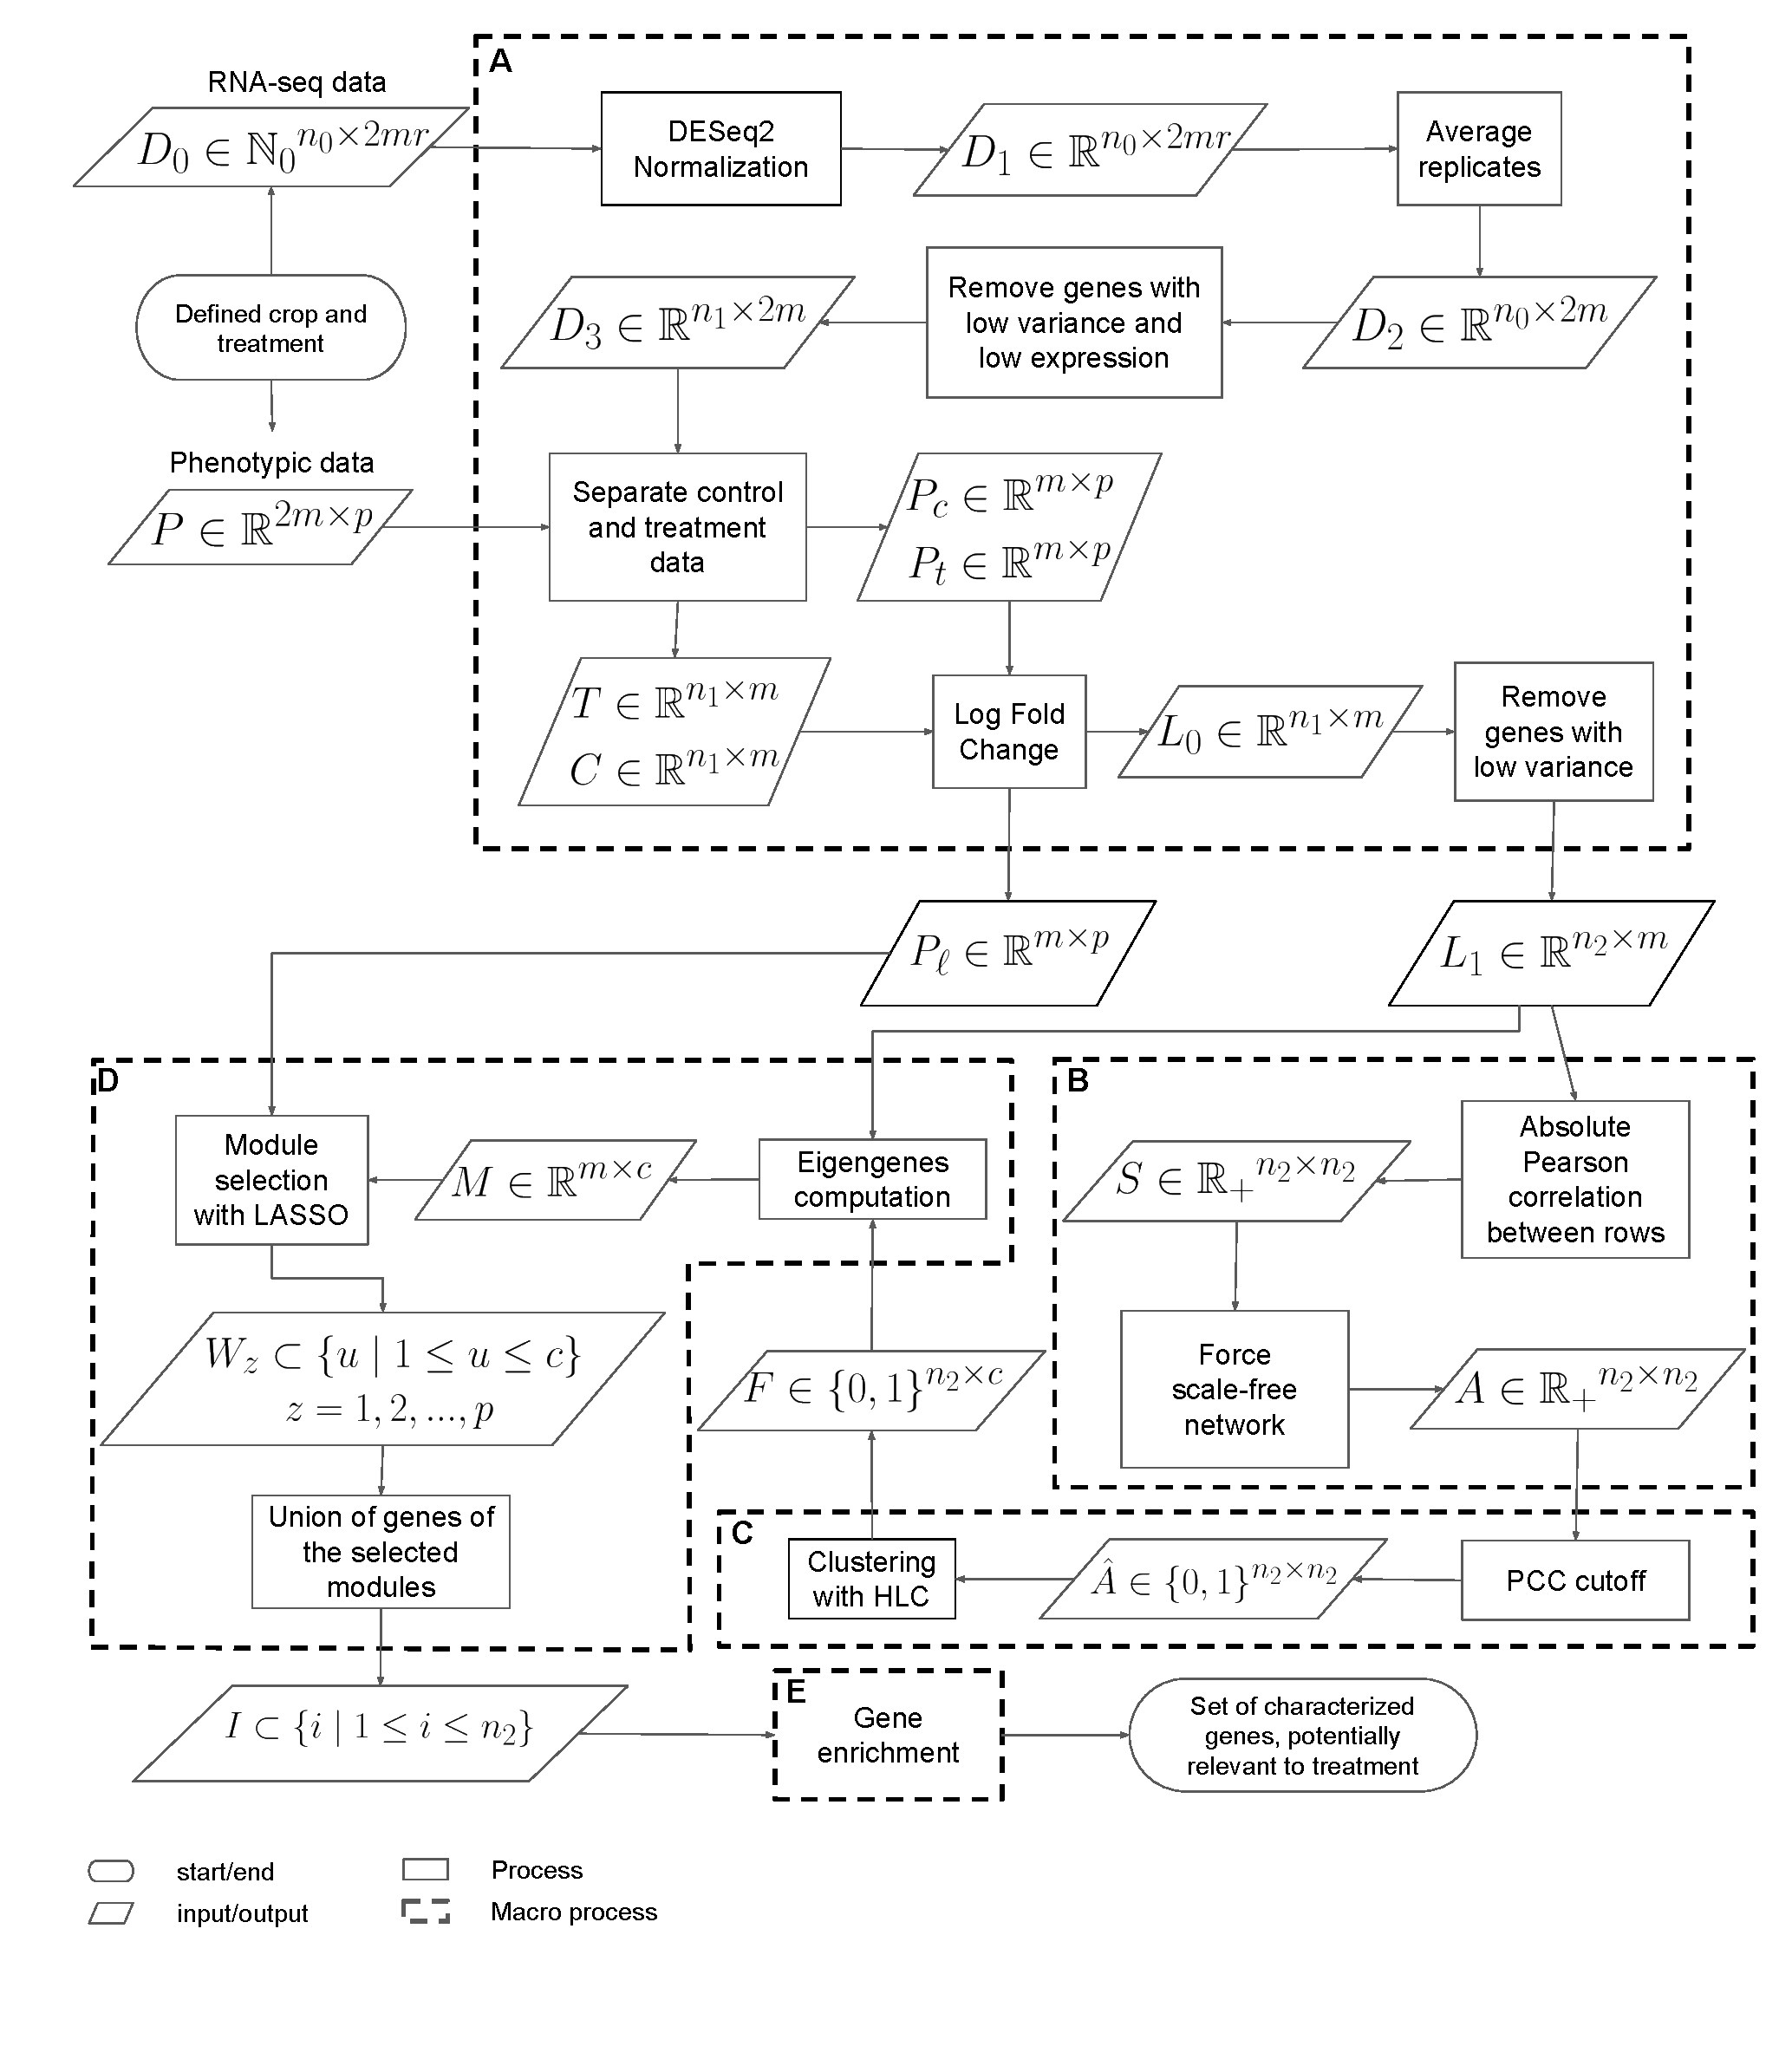
\includegraphics[clip,width=1\textwidth]{figures/flow_chart_2.pdf}
  \caption{The proposed workflow comprising five macro-steps:
    A.~Data pre-processing, B.~Co-expression network
    contruction, C.~Co-expression module identification,
    D.~Modules association to phenotypic traits, and
    E.~Genes enrichment.}
  \label{fig:flow_chart}
\end{figure}

\subsection{Data pre-processing}
The goal of the data pre-processing stage is to build matrices $P_ell$ and $L_1$ representing, respectively, the changes in phenotypic values and expression levels between control and treatment condition, from RNA-seq and phenotypic data found in matrices $D_0$ and $P$, respectively.

The RNA-seq data cannot be directly interpreted. Therefore, a normalization process is applied to deal with the problem of possible biases affecting the quantification of results. The suggested normalization technique for correcting library size and RNA composition bias is DESeq2 \cite{love2014moderated}. The normalized data is represented as a matrix $D_1 \in \mathbb{R}^{n_0 \times 2mr}$, and the biological replicates of each genotype are averaged and represented as a matrix $D_2 \in \mathbb{R}^{n_0 \times 2m}$. The genes exhibiting low variance or low expression are removed from $D_2$, thus identifying a subset of size $n_1 \leq n_0$ of the original genes. The control and treatment data is separated into the matrices $C\in \mathbb{R}^{n_1 \times m}$ and $T\in \mathbb{R}^{n_1 \times m}$, respectively. The matrix entries $c_{ij}$ in $C$ and $t_{ij}$ in $T$ represent, respectively, the normalized expression level of gene $i$ in accession $j$. Control and treatment data is also separated from phenotypic data $P$, obtaining the $P_c$ and $P_t$ matrices of dimensions $m \times p$.

In the above configuration, the changes in expression levels and phenotypic values, between control and treatment conditions, are measured in terms of logarithmic ratios. In the case of expression levels, the log ratios are represented in the Log Fold Change matrix $L_0 \in \mathbb{R}^{n_1 \times m}$, where $\ell_{ij}=\log_2 (t_{ij}/c_{ij})$. Similarly, the log ratios of the phenotypic data are computed and represented in the $P_\ell \in \mathbb{R}^{m \times p}$ matrix.

The final step of the data pre-processing is to filter $L_0$ by removing rows (e.g., genes) with low variance in the differential expression patterns, obtaining a new matrix $L_1$ of dimensions $n_2 \times m$, with $n_2 \leq n_1$.

\subsection{Co-expression network construction}

A gene co-expression network connect genes with similar expression patterns across biological conditions. The purpose of this stage is to describe how to build the co-expression network $A$ from the Log Fold Change matrix $L_1$, capturing the relationship between genes according to the change in expression levels between the two studied conditions. These co-expression patterns are meaningful for the identification of genes not yet associated with the response to the treatment condition.

The Log Fold Change matrix $L_1$ is used to build the co-expression network following the first two steps of the WGCNA methodology~\cite{langfelder2008wgcna}. First, the level of concordance between gene differential expression profiles across samples is measured. To this end, the absolute value of the Pearson correlation coefficient is used as the similarity measure between genes and the resulting values are stored in the similarity matrix $S\in \mathbb{R_{+}}^{n_2 \times n_2}$. Second, the matrix $S$ is transformed into and adjacency matrix $A \in \mathbb{R_+}^{n_2\times n_2}$ where each entry $a_{ij} = (s_{ij})^\beta $ encodes the connection strength between each pair of genes. In other words, the elements of the adjacency matrix are the similarity values up to the power $\beta > 1$ so the degree distribution will fit a scale-free network. These networks contain many nodes with very few connections and a small number of hubs with high connections. In a strict scale-free network the logarithm of $P(k)$ (i.e., the probability of a node having degree $k$) is approximately inversely proportional to the logarithm of $k$ (i.e., the degree of a node). So the parameter $\beta$ is chosen as the smallest value of $\beta$ such that the $R^2$ of the linear regression between $log_{10}(p(k))$ and $log_{10}(k)$ is close to $1$ (e.g., $R^2 > 0.85$). 

\subsection{Co-expression module identification}

Next step in the workflow is to identifying communities (also called modules)
from the co-expression network structure and dynamics represented in $A$. 
The idea is to cluster genes with similar patterns of differential
expression change. Membership in these modules may overlap in 
biological contexts, because modules may be related to specific 
molecular, cellular or tissue functions and the biological components
(i.e. genes) may be involved in multiple functions. Thus, unlike WGCNA, the adjacency matrix $A$ is used to detect overlapping (rather than non-overlapping) communities, using the Hierarchical Link Clustering (HLC) algorithm (see section~\ref{sec.prelim}).

As a prelimiary step, matrix $A$ is transformed, into an unweighted network $\hat{A} \in \{0,1\}^{n_2 \times n_2}$ before applying the clustering algorithm. To this end, the Pearson Correlation Coefficient (PCC) cutoff is determined using the approach described in~\cite{aoki2007approaches}. The number of nodes, edges, and the network density is determined for different PCC cutoffs. Around the most biological relevant PCC cutoff, the number of nodes presents a linear decrease, and the density of the network reaches its minimum, while below this value the number of edges rapidly increases. Considering this, a cutoff is selected such that gene pairs which have a correlation score higher than the threshold are considered to have significant co-expression relationship. Above the cutoff, the entries of matrix $A$ become $1$ and below the cutoff $A$ values becomes $0$. The application of the HLC algorithm organizes the $n_2$ genes of matrix $\hat{A}$ into $c$ modules, where each gene can belong to one, multiple, or no module at all. This information is represented as an affiliation matrix $F \in \{0,1\}^{n_2 \times c}$, where $f_{iu} = 1$ if node $i$ is member of module $u$.

\subsection{Module association to phenotypic traits}

To identify the most relevant groups (modules) of genes, associated
with the phenotypic response to a specific treatment in an organism,
the proposed workflow uses a LASSO based approach. Each module is
represented by an eigengene, which is defined as the first principal
component of such module. An eigengene can be thought of as an average
differential expression profile for each community: it is computed
from the Log Fold Change Matrix $L_1$ and the affiliation matrix
$F$. Given a module $u$, the affiliation matrix is used to identify
the genes belonging to $u$ and then the corresponding rows of the
matrix $L_1$ are selected to compute the first principal component of
$u$. Each principal component becomes a column of the matrix $M \in
\mathbb{R}^{m \times c}$.
These profiles are associated with each phenotypic trait using 
the least absolute shrinkage and selection operator (LASSO). 
In this context, the eigengenes (i.e., the columns of $M$) act as regressor variables
and each phenotypic trait (i.e., each column of $P_\ell$) is used as an outcome variable.

The output after applying LASSO is a set $W_z$ of modules for each
phenotypic trait $z$, where $W_z \subset \{u \mid 1 \leq u \leq c\}$ for
$z= 1,2,..,p$. The target genes $I$ for downstream analysis, which may
be important in the treatment response, are the union of genes belonging
to the selected modules, that is $I = \cup_{z=1}^{p} W_z$, where
$I \subset \{i \mid 1 \leq i \leq n_2\}$.

\subsection{Gene Enrichment}

The goal of this final stage of the process is to characterize the
genes identified in previous stage with additional information, helping to elucidate their
possible behavior and role in the response to the studied treatment.

A simple analysis to made with the selected genes is to identify the
differentially expressed genes in set $I$. That is, to select those genes
in $I$ having an absolute value of the log fold change of at least $2$
($|\ell_{ij}|\geq 2$) for at least one sample. This
represents genes level of expression is quadrupled (up or down)
from control to treatment condition; these genes are
strong candidates for treatment responsive genes.

Also functional category enrichment can be done by, e.g., searching for gene ontology annotations in databases such as QuickGO~\cite{binns2009quickgo}. Such annotations 
can provide evidence of biological implications of the target genes in
the treatment-tolerance mechanisms. Furthermore, QuickG0 can be used to identify genes with reported protein products, which can be used to perform additional relevant
analysis reviewing their reported protein-protein interactions in other databases, such as STRING~\cite{szklarczyk2016string}. The interactions include direct (physical) and indirect (functional) associations; they stem from computational prediction, from knowledge
transfer between organisms, and from interactions aggregated from
other (primary) databases. This information can give new insight on how the
selected genes are involved in functional pathways that can be related
with the treatment of interest.
